\chapter{Logistic Regression}


\section{Classification and Hypothesis }
\begin{itemize} 
    \item A \textbf{sigmoid function} is a mathematical function having a characteristic \textbf{s-shaped} curve. A common example of a sigmoid function is the \textbf{logistic function} shown in the figure \ref{fig:sigmoid}.
    \begin{equation}
        g(z) = \frac{1}{1+e^{-z}}
    \end{equation}

    \item When $z \geq 0$, the output will be greater than or equal 0.5.
    \begin{figure}[!htbp]\label{fig:sigmoid}
        \centering
        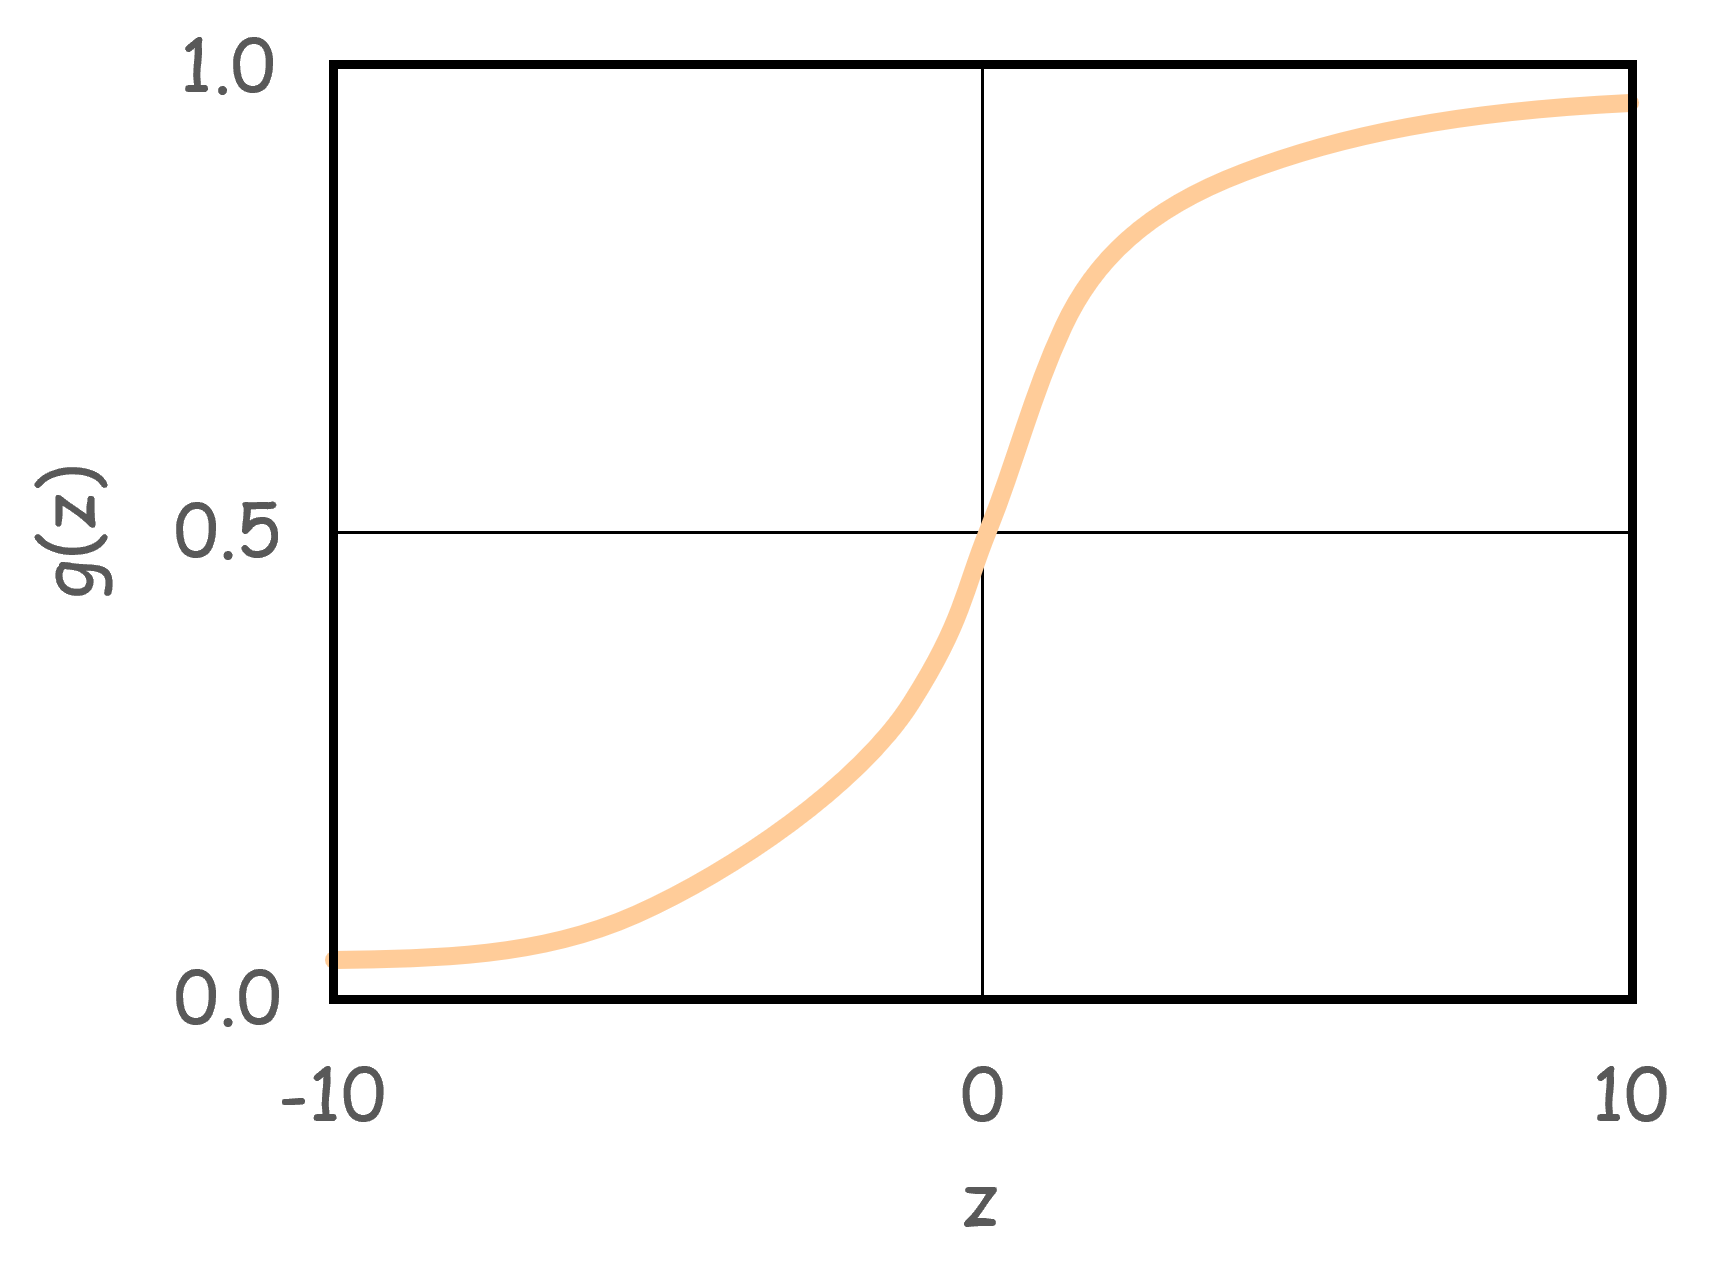
\includegraphics[width=2.8in]{./images/sigmoid.png}
        \caption{Logistic function}
    \end{figure}

    \item For a \textbf{binary classification problem}, $y \in (0,1)$, change the form of the hypothesis  $h^{(i)}$ as a logistic function to satify $0 \leq h^{(i)} \leq 1$. Substitute z into $\mathbf{x}^{(i)}\theta$
    \begin{equation}
        h^{(i)} = \frac{1}{1+e^{-\mathbf{x}^{(i)}\theta}}
    \end{equation}
    where
    \begin{equation}
        \mathbf{x}^{(i)} = 
        \left[
            \begin{array}{cccc}
                x_0^{(i)} & x_1^{(i)} & \dots & x_n^{(i)}  
            \end{array}
        \right],
        \theta = 
        \left[
            \begin{array}{c}
                \theta_0 \\ \theta_1 \\ \vdots \\ \theta_n
            \end{array}
        \right]
    \end{equation}
    Let
    \begin{eqnarray}
        \mathbf{h} = 
        \left[
        \begin{array}{c}
            h^{(1)} \\ h^{(2)} \\ \vdots \\ h^{(m)}
        \end{array}
        \right]
    \end{eqnarray}
    \item The hypothesis $h^{(i)}$ will give the \textbf{probability}. For example, $h^{(i)}=0.7$ means the probability of 70\% that the output is ``1''.
    \begin{equation}
        h^{(i)} = P(y=1|x;\theta) = 1 - P(y=0|x;\theta)
    \end{equation}
\end{itemize}


\section{Cost Function}
\begin{itemize}
    \item If the cost function of a logistic function is used the same as for linear regression, it will cause many local optima. (Not a \textbf{convex} function)
    Instead, the cost function for logistic regression looks like:
    \begin{equation}
        \begin{split}
            J(\theta) = \frac{1}{m}\sum_{i=1}^{m}{L(h^{(i)},y^{(i)})}\\
        \end{split}
    \end{equation}
    
    where,
    \begin{equation}
        L(h^{(i)},y^{(i)}) =
        \left\{
        \begin{array}{ll}
            -\log{(h^{(i)})}   & \mbox{if $y^{(i)}=1$}\\
            -\log{(1-h^{(i)})} & \mbox{if $y^{(i)}=0$}
        \end{array}
        \right.
    \end{equation}
    
    These two cases are shown as Figure \ref{fig:logisticCostttt}. 
    \begin{figure}[!htbp]\label{fig:logisticCostttt}
        \centering
        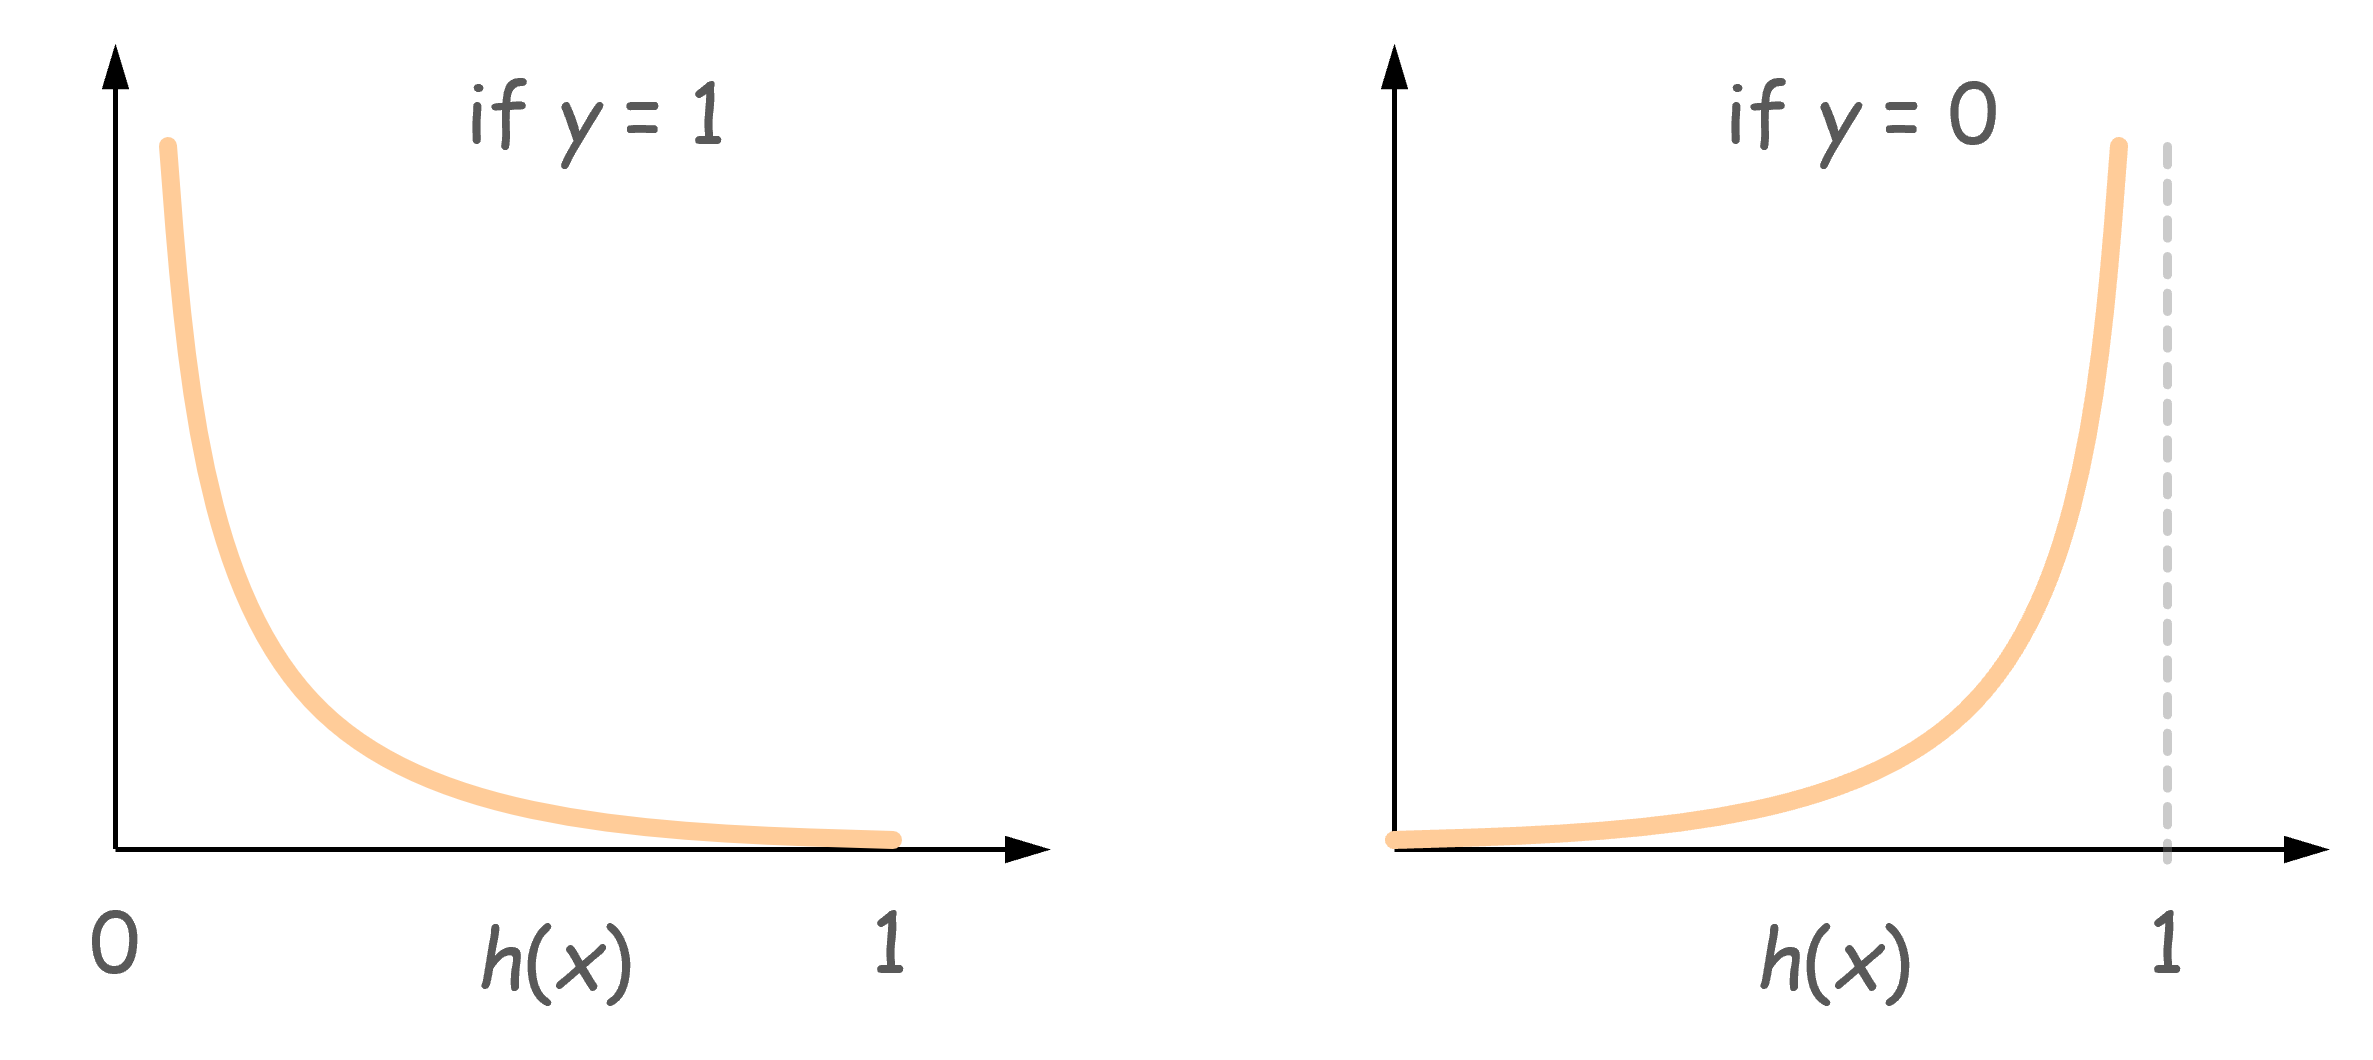
\includegraphics[width=3.2in]{./images/logisticCost.png}
        \caption{Cost of logistic function}
    \end{figure}

    The function $L$ can be compressed into one case
    \begin{equation}
        L(h^{(i)},y^{(i)}) = -y^{(i)}\log{(h^{(i)})}-(1-y^{(i)})\log{(1-h^{(i)})}
    \end{equation}
    
    Thus, the entire cost function as follows:
    \begin{equation}
        J(\theta) = -\frac{1}{m} \sum_{i=1}^{m} \left[ {y^{(i)}\log{(h^{(i)})}+(1-y^{(i)})\log{(1-h^{(i)})}} \right]
    \end{equation}
    
    A vectorized implementation is:
    \begin{equation}
        J(\theta) = -\frac{1}{m} \left( \mathbf{y}^T\log{(\mathbf{h})} + \mathbf{(1-y)}^T\log{(\mathbf{1-h})} \right)
    \end{equation}
\end{itemize}


\section{Gradient Descent}
\begin{itemize}
    \item Repeat until convergence
    \begin{equation}
        \begin{split}
            \theta_j &\coloneqq \theta_j - \alpha \frac{\partial}{\partial\theta_j}J\left(\theta\right)\\
            &\coloneqq \theta_j - \frac{\alpha}{m} \sum_{i=1}^{m}\left[\left(h^{(i)}-y^{(i)}\right)x^{(i)}_j\right]
        \end{split}
    \end{equation}
    for $j=0,1,\dots,n$. 
    \item Surprisingly, the update rule is the same as the one derived in linear regression. As a result, the same gradient descent formula can be used for logistic regression as well.
    
    \item
    \begin{proof}
        The derivative for the cost function is
        \begin{equation}
            \frac{\partial J(\theta)}{\partial\theta_j} = \frac{-1}{m} \sum_{i=1}^{m} \frac{\partial}{\partial h^{(i)}} L\left(h^{(i)},y^{(i)}\right) \frac{\partial h^{(i)}}{\partial \theta_j}
        \end{equation}
        
        Compute the first derivative term, consider the base number of logarithm is $e$
        \begin{equation}
            \begin{split}
                \frac{\partial}{\partial h^{(i)}} L\left(h^{(i)},y^{(i)}\right)  &= y^{(i)} \frac{\partial}{\partial h^{(i)}} \log\left(h^{(i)}\right) + \left(1-y^{(i)}\right) \frac{\partial}{\partial h^{(i)}} \log\left(1-h^{(i)}\right)\\
                &= \frac{y^{(i)}}{h^{(i)}} - \frac{1-y^{(i)}}{1-h^{(i)}}\\
                &= - \frac{h^{(i)}-y^{(i)}}{{h^{(i)}}\left(1-h^{(i)}\right)}
            \end{split}
        \end{equation}
        
        And the second derivative term,
        \begin{equation}
            \begin{split}
                \frac{\partial h^{(i)}}{\partial \theta_j} &= \frac{\partial}{\partial \theta_j} \frac{1}{1+e^{-\mathbf{x}^{(i)}\theta}}
            \end{split}
        \end{equation}
        
        Let
        \begin{equation}
            \begin{split}
                \alpha &= 1 + e^{-\mathbf{x}^{(i)\theta}}\\
                \beta  &= -\mathbf{x}^{(i)}\theta
            \end{split}
        \end{equation}
        
        Then
        \begin{equation}
            \begin{split}
                \frac{\partial h^{(i)}}{\partial \theta_j} &= \frac{\partial h^{(i)}}{\partial \alpha} \frac{\partial \alpha}{\partial \beta} \frac{\partial \beta}{\partial \theta_j}\\
                &= \frac{-1}{\left(1 + e^{-\mathbf{x}^{(i)\theta}}\right)^2} e^{-\mathbf{x}^{(i)\theta}} \left(-x^{(i)}_j\right)\\
                &= \frac{1}{1+e^{-\mathbf{x}^{(i)\theta}}} \left(\frac{-e^{-\mathbf{x}^{(i)\theta}}}{1+e^{-\mathbf{x}^{(i)\theta}}}\right)\left(-x^{(i)}_j\right)\\
                &= h^{(i)} \left(1-h^{(i)}\right) \left(-x^{(i)}_j\right)
            \end{split}
        \end{equation}
        
        So
        \begin{equation}
            \frac{\partial J(\theta)}{\partial\theta_j} = \frac{-1}{m} \sum_{i=1}^{m} \left[\left(h^{(i)}-y^{(i)}\right)x^{(i)}_j\right]
        \end{equation}
    \end{proof}

    \item The vectorized implementation is
    \begin{equation}
        \mathbf{\theta} \coloneqq \mathbf{\theta} - \frac{\alpha}{m}\mathbf{X}^T\left(\mathbf{h}-\mathbf{y}\right)
    \end{equation}


\end{itemize}


\section{Decision Boundary}
\begin{itemize}
    \item After the optimization of parameters $\theta_j$ where $j=0,\dots,n$, the decision boundary is
    \begin{equation}
        \theta_0 x_0 + \theta_1 x_1 + \dots + \theta_n x_n = 0
    \end{equation}
    
    \item For example. If
    \begin{equation}
        \theta = 
        \left[\begin{array}{ccc} -3 & 1 & 1 \end{array}\right]^T
    \end{equation}
    
    The decision boundary is
    \begin{equation}
        -3 x_0 + x_1 + x_2 = 0
    \end{equation}

    For those points located at the upper-right side of the decision boundary, the predictions are $y=1$.
    On the contrary, for those points located at the lower-left side are $y=0$.
    \begin{figure}[!htbp]
        \centering
        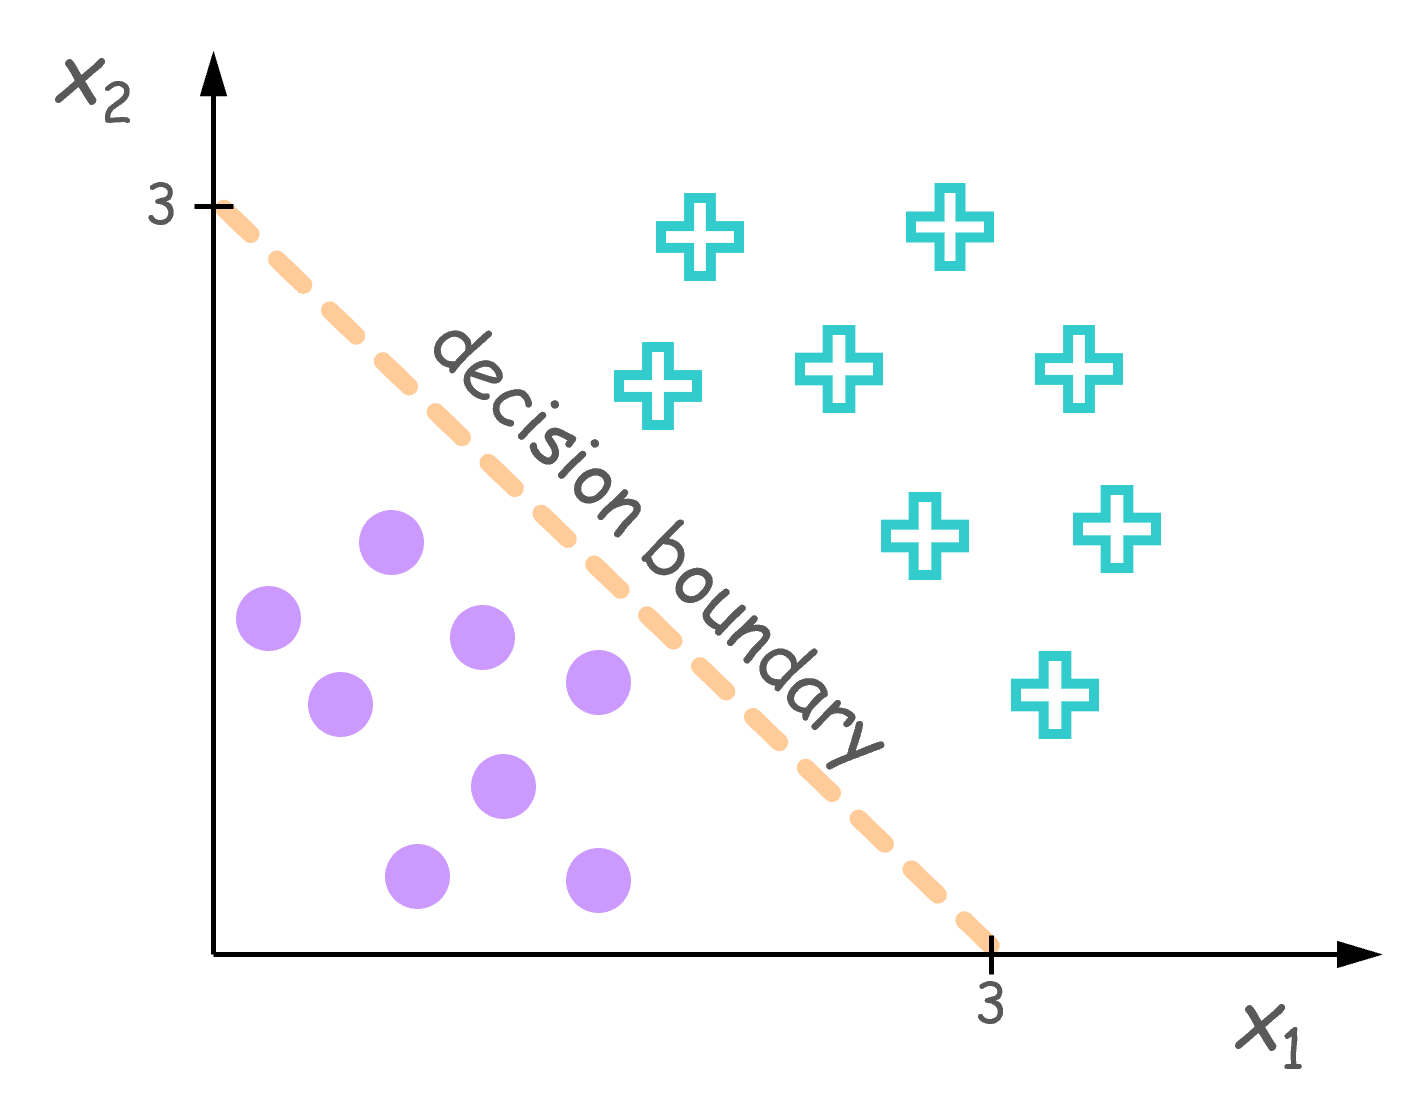
\includegraphics[width=2.6in]{./images/decision boundary.png}
        \caption{Logistic function}
    \end{figure}
    
    \item An non-linear decision boundary can also be created by adding polynomial terms in the array of parameters, such as
    \begin{equation}
        \theta = 
        \left[\begin{array}{ccccc} \theta_0 & \theta_1 & \theta_2 & \theta_1^2 & \theta_2^2 \end{array}\right]^T
    \end{equation}
    
    For this case, the optimized parameters would be like
    \begin{equation}
        \theta = 
        \left[\begin{array}{ccccc} -1 & 0 & 0 & 1 & 1 \end{array}\right]^T
    \end{equation}
    
    Then the decision boundary is
    \begin{equation}
        -1 + x_1^2 + x_2^2 = 0
    \end{equation}

    The prediction would be
    \begin{equation}
        y = \left\{\begin{aligned}
            1 &\text{, for } x_1^2 + x_2^2 \geq 1\\
            0 &\text{, for } x_1^2 + x_2^2 < 1
        \end{aligned}\right.
    \end{equation}

    \begin{figure}[!htbp]
        \centering
        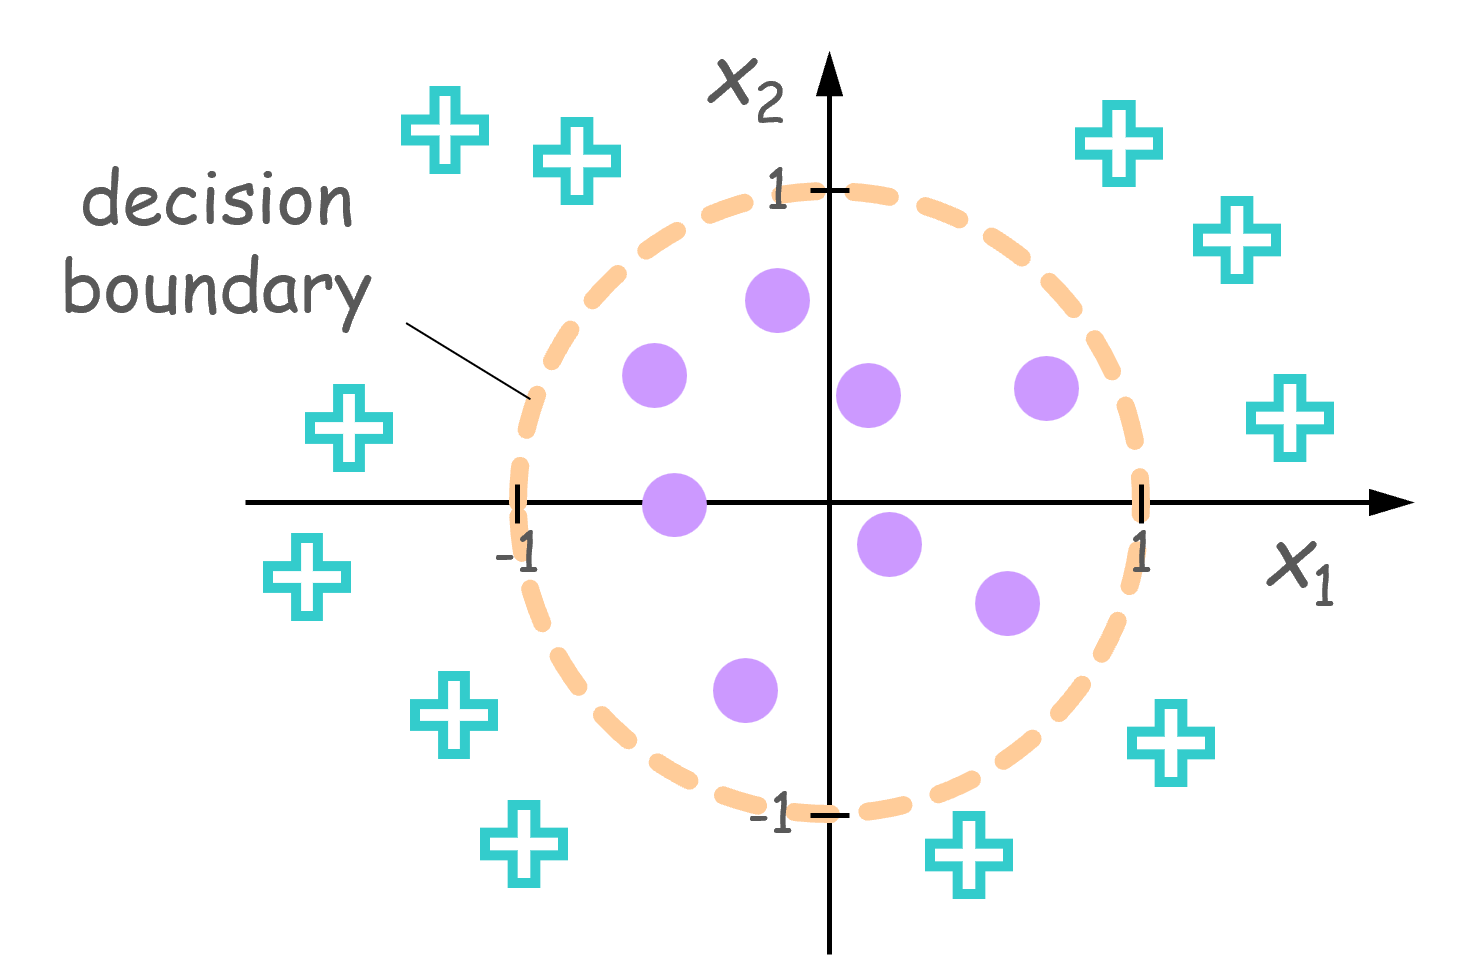
\includegraphics[width=2.6in]{./images/decision boundary_nonlinear.png}
        \caption{Logistic function}
    \end{figure}
    
\end{itemize}